\section{Analysis}

The goal is to build an automatic analyzer which takes as input an arbitrary program and an arbitrary property such that the analyzer can answer if the property holds or not. But this problem is undecidable, so we have to make some sacrifices. We only want the analyzer to decided if the property holds for sure.

\begin{center}
	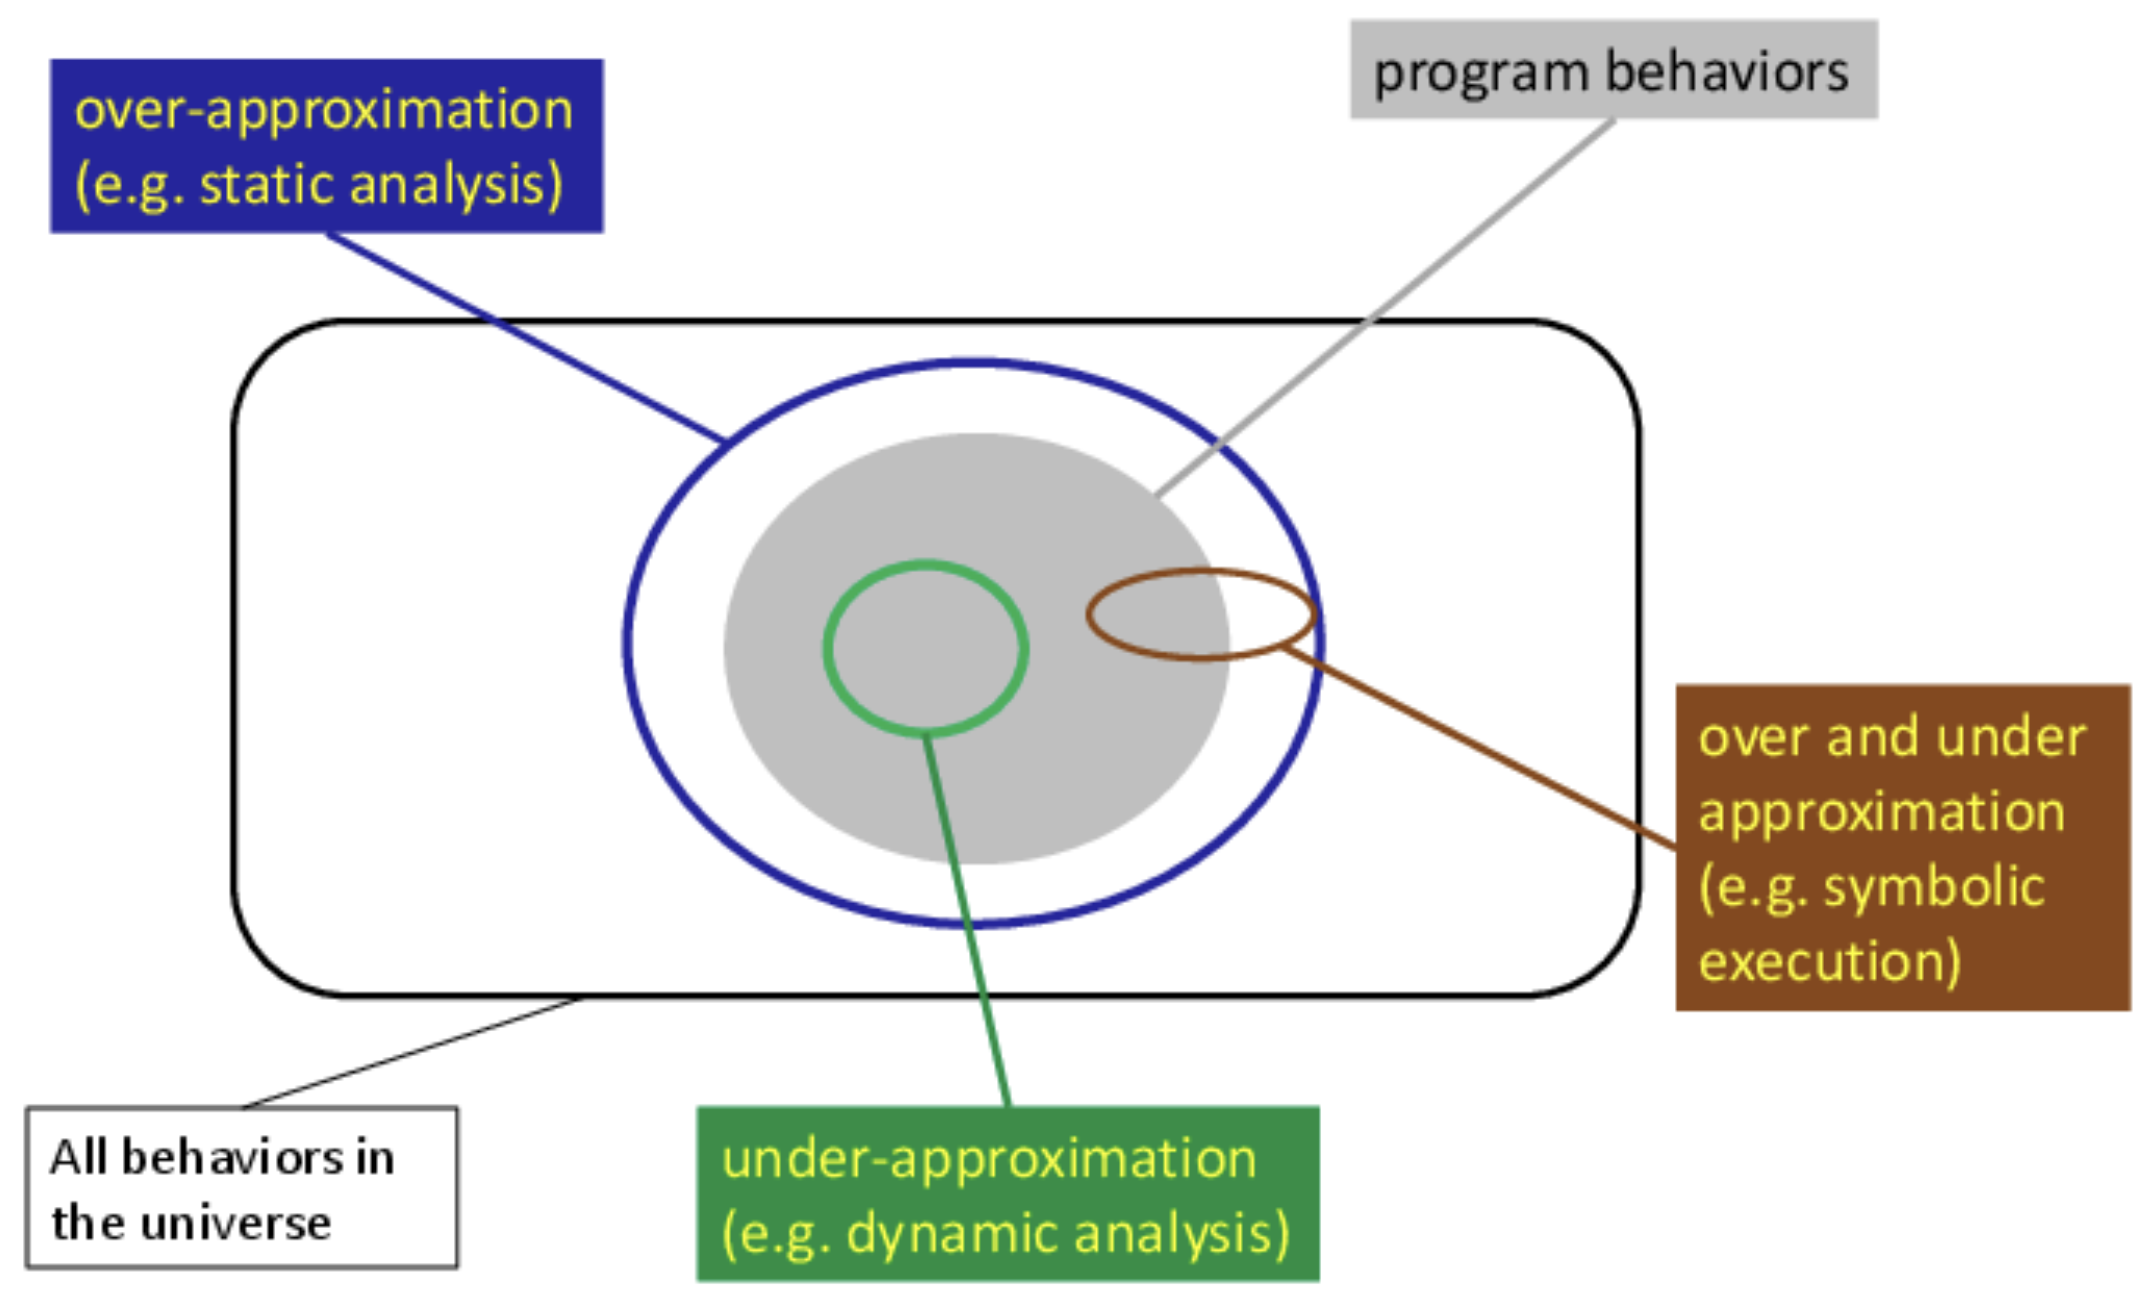
\includegraphics[width=0.8\columnwidth]{assets/program_behavior}
\end{center}

Static program analysis can run the program without giving a concrete input and does not need any manual annotations such as loop invariants.


\subsection{Abstract Interpretation}

Abstract interpretation works by:
\begin{enumerate}
	\item Select / define an abstract domain
	\item Define abstract semantics for the language w.r.t. to the domain
	\item Iterate abstract transformers over the abstract domain until a fixed point is reached
\end{enumerate}

It is important to remember that abstract transformers are defined per programming language once and for all, and not per program. A correct abstract transformer should always produce results that are a superset of what a concrete transformer would produce. In general it is easy to be sound and imprecise, being sound and precise is hard. \\

One example for this type of interpretation uses the interval domain given by:
\begin{center}
	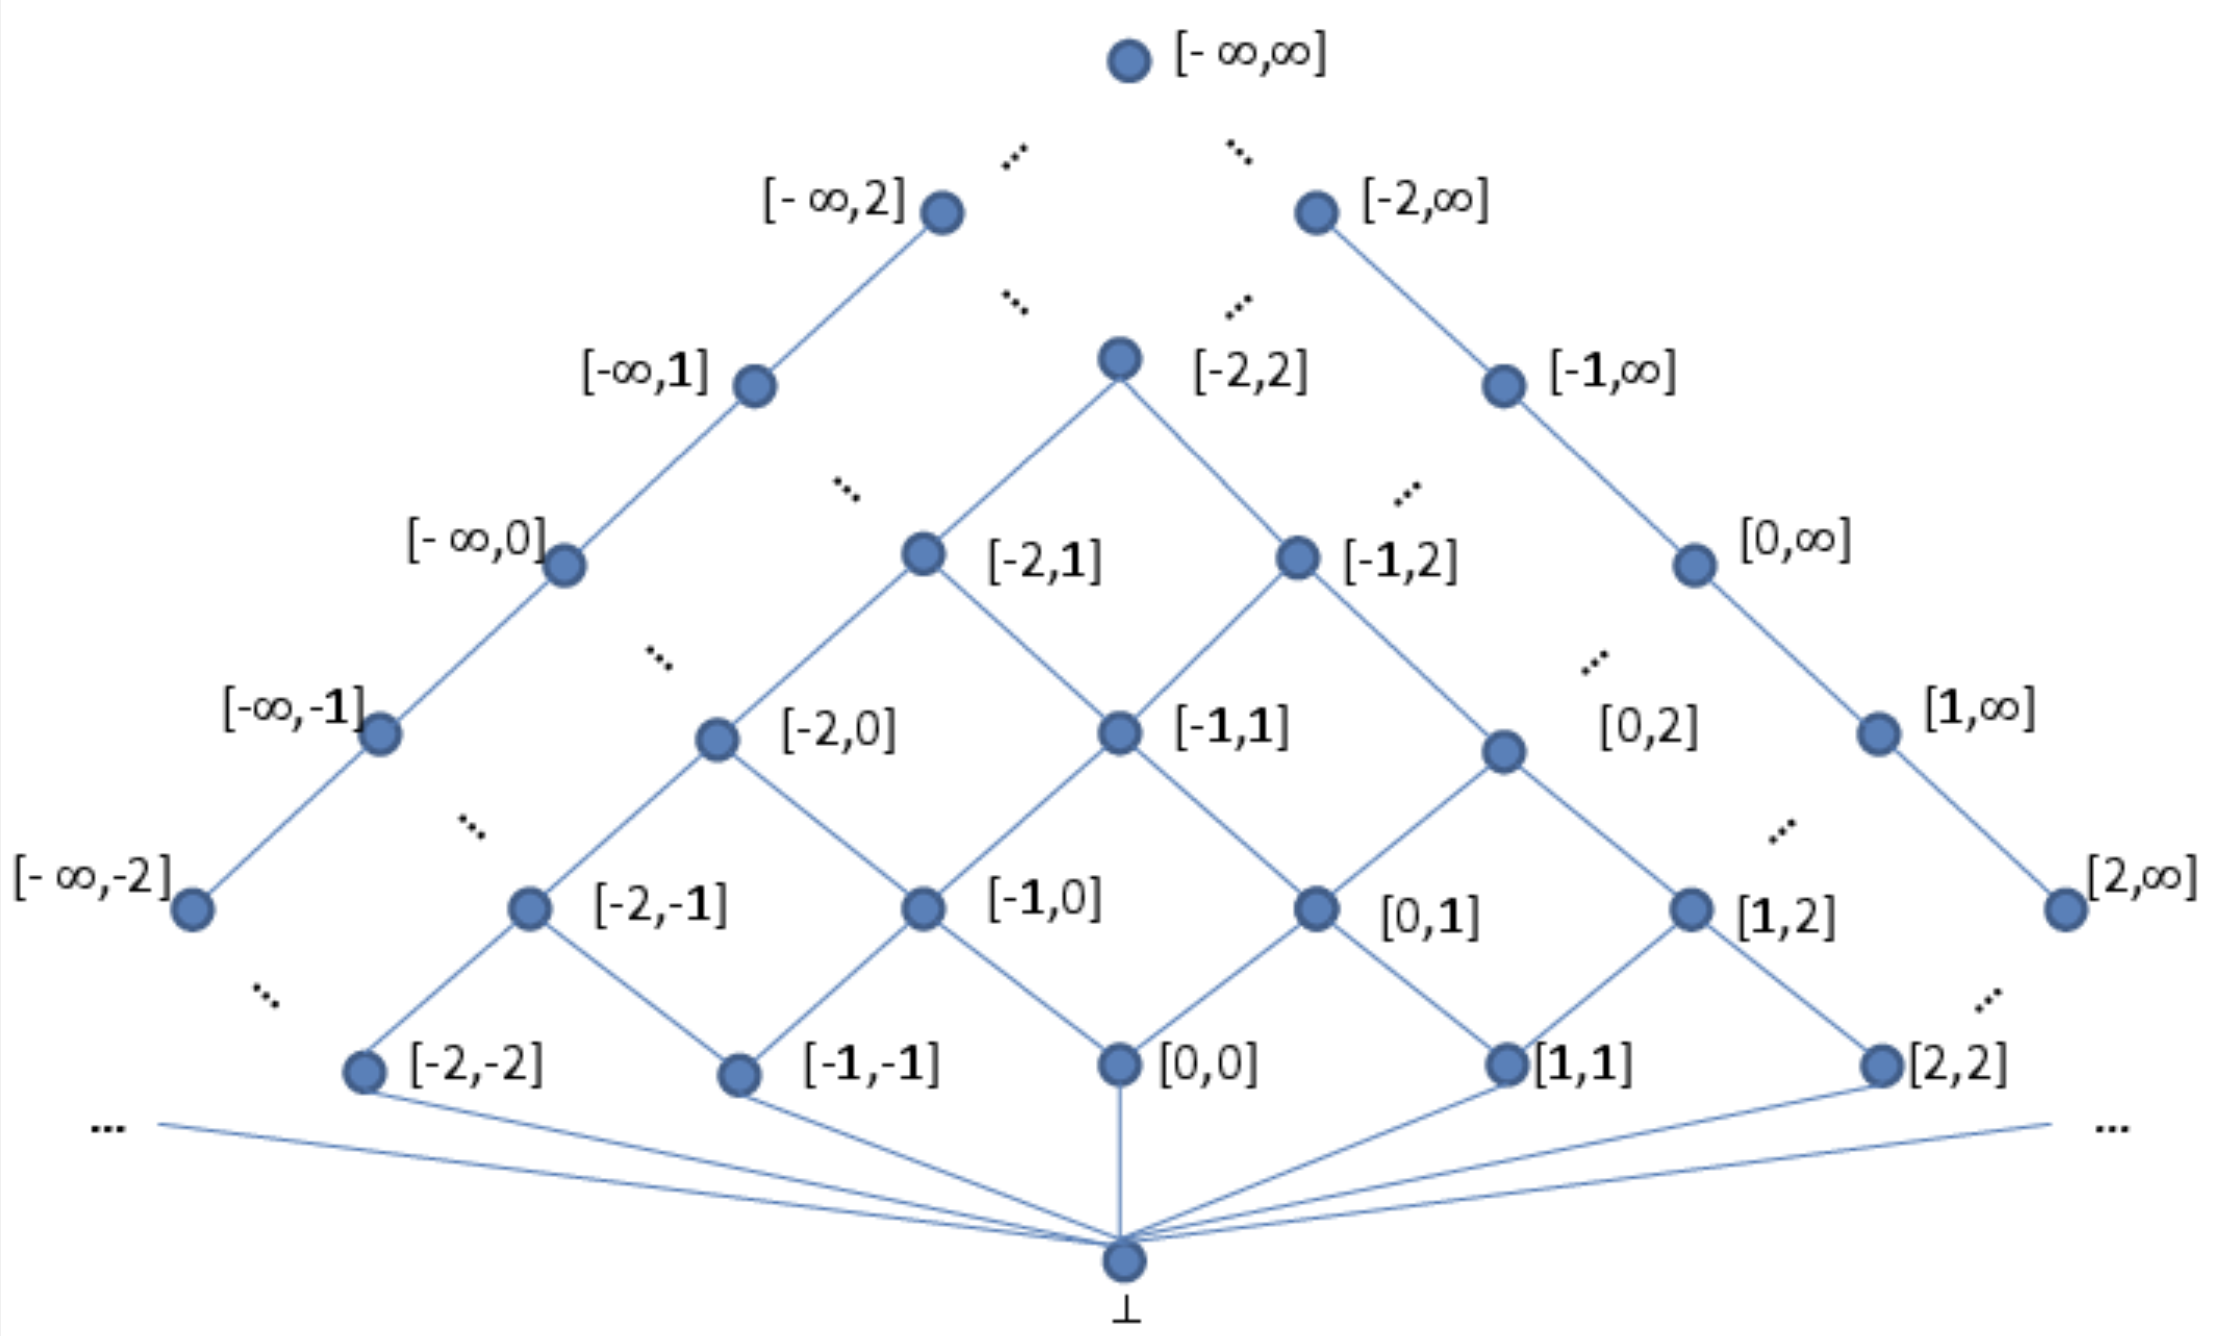
\includegraphics[width=0.8\columnwidth]{assets/interval_domain}
\end{center}

When we have two abstract elements $A$ and $B$, we can join them to produce their (least) upper bound, denoted by $A \sqcup B$. For this we have to define the join operation. \\

With the interval abstraction we can have cases where we cannot reach a fixed point, e.g. loop that always counts up. To fix this we introduce the widening operator, it ensures termination at the expense of precision. If the bound of an interval is increasing, we simply go to $\infty$ instead of widening the interval multiple times.


\subsection{Mathematical Concepts}

\subsubsection{Structures}

A partial order is a binary relation $\sqsubseteq \; \subseteq \; L \times L$ on a set $L$ with the properties of being reflexive, transitive and anti-symmetric. The intuition is that it captures implications between facts. Later, we will say that if $p \sqsubseteq q$, then $p$ is more precise than $q$. Given a poset, we can construct a Hasse diagram. \\

Given a poset $(L, \sqsubseteq)$, an element $\bot \in L$ is called the least element if it is smaller than all other elements of the poset. The greatest element $\top$ is defined analogous. The least and greatest elements may not exist, but if they do they are unique. \\

Given a poset $(L, \sqsubseteq)$ and $Y \subseteq L$, $u \in L$ is an upper bound of $Y$ if $\forall p \in Y: p \sqsubseteq u$. $\bigsqcup Y \in L$ is a least upper bound of $Y$ if it is an upper bound of $Y$ and $\bigsqcup Y \sqsubseteq u$ whenever $u$ is another upper bound of $Y$. We define the lower bound and greatest lower bound analogously. \\

A complete lattice $(L, \sqsubseteq, \bigsqcup)$ is a poset where $\bigsqcup Y$ and $\bigsqcap Y$ exist for any $Y \subseteq L$. The interval domain from above is a complete lattice.

\subsubsection{Functions}

A function $f: A \to B$ between two posets $(A, \sqsubseteq)$ and $(B, \leq)$ is increasing (monotone) if: 
$$\forall a, b \in A: a \sqsubseteq b \Rightarrow f(a) \leq f(b)$$

For a poset $(A, \sqsubseteq)$, a function $f: A \to A$, and element $a \in A$, $a$ is a fixed point iff $f(a) = a$. Further $a$ is a post-fixedpoint iff $f(a) \sqsubseteq a$. The set of all fixed points is denoted by Fix(f) and the set of all post-fixedpoints is denoted by Red(f). \\

For a poset $(A, \sqsubseteq)$ and a function $f: A \to A$, we say that $\text{lfp} \sqsubseteq f \in A$ is a least fixed point of $f$ if $\text{lfp} \sqsubseteq f$ is a fixed point and $\forall a \in A: a = f(a) \Rightarrow \text{lfp} \sqsubseteq f \sqsubseteq a$.

\begin{center}
	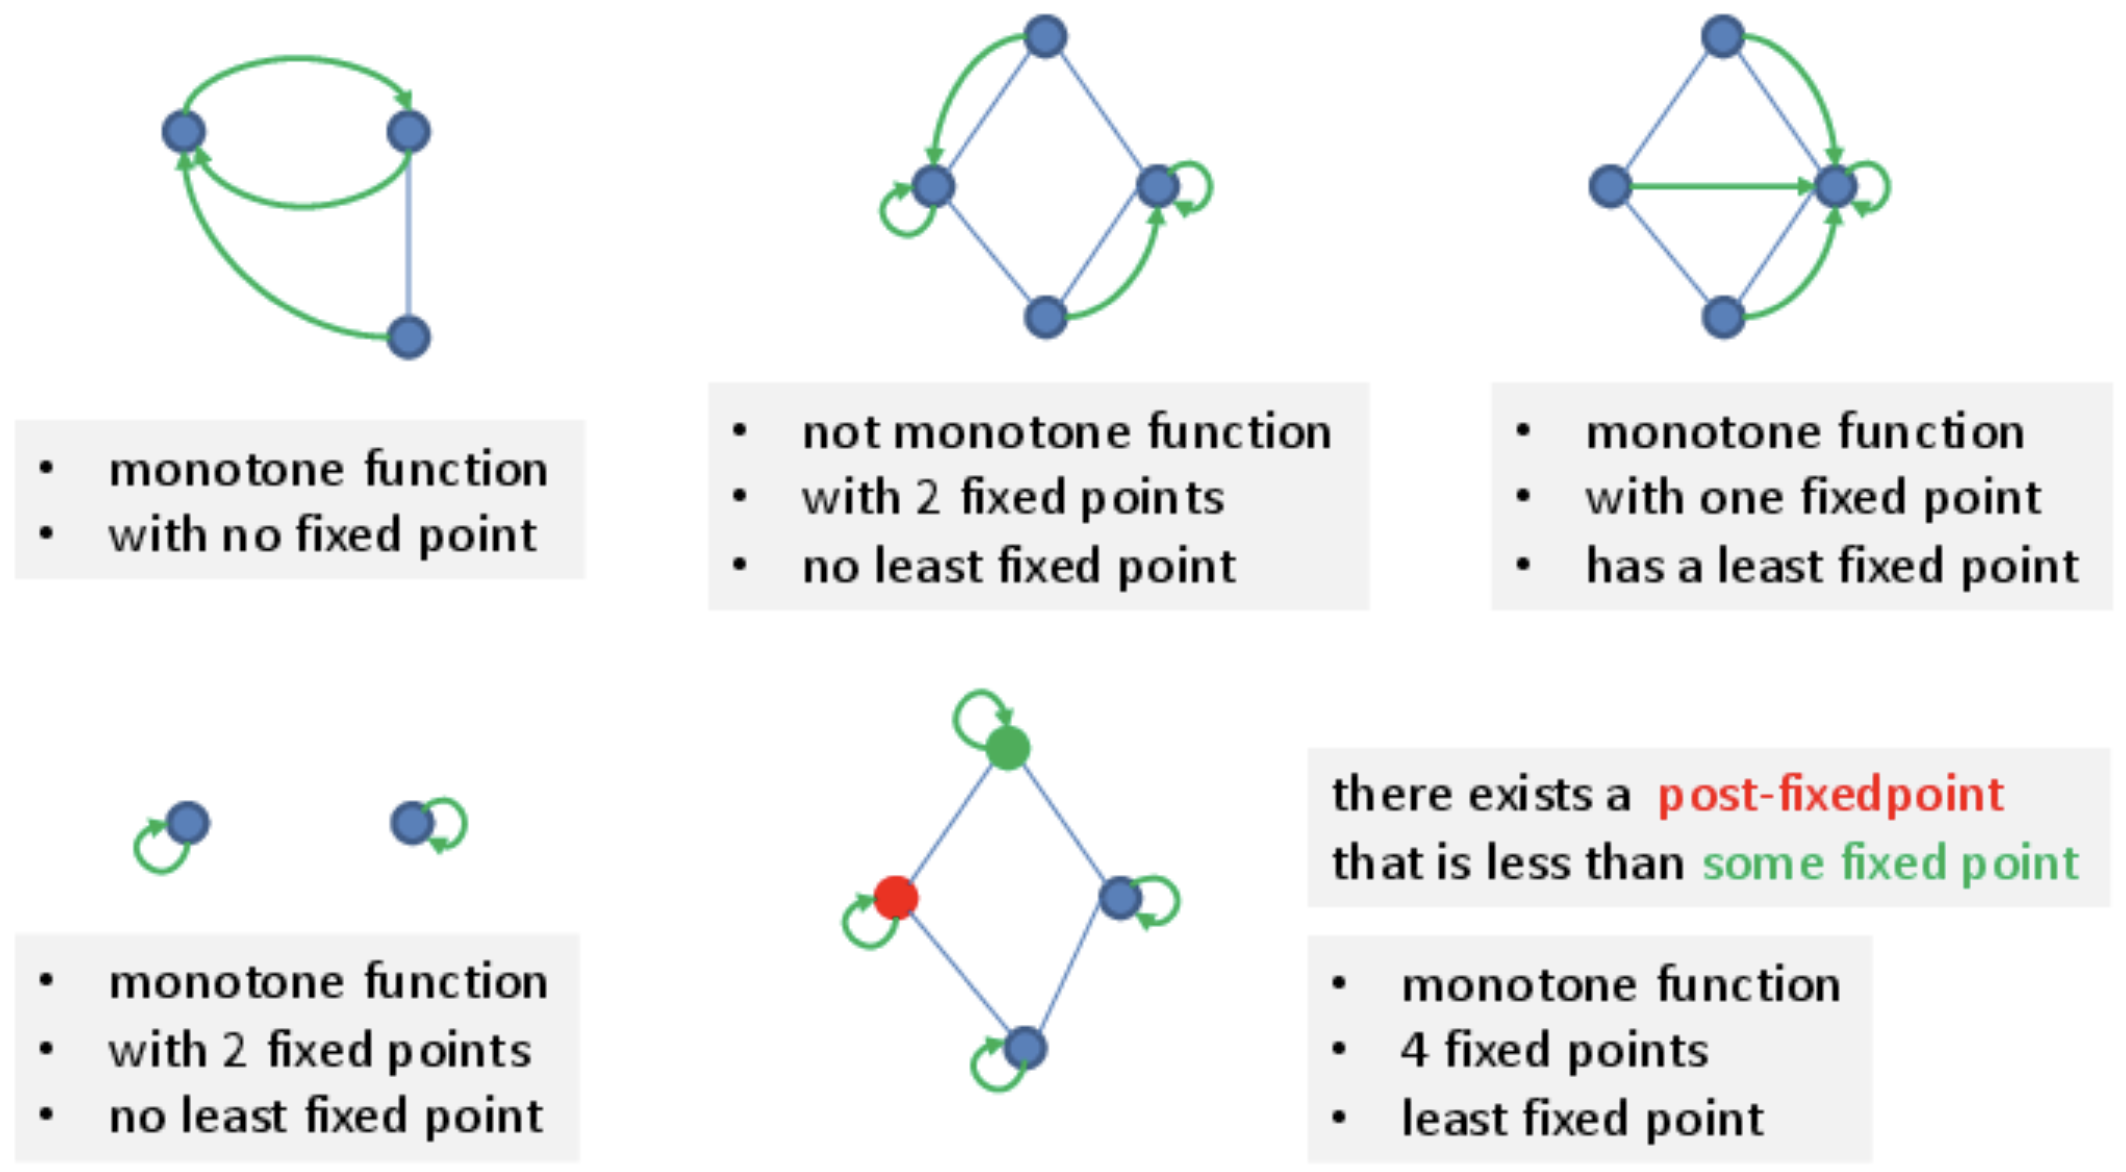
\includegraphics[width=\columnwidth]{assets/fixed_points}
\end{center}

If $(A, \sqsubseteq), \bigsqcup, \bigsqcap, \bot, \top)$ is a complete lattice and $f: A \to A$ is a monotone function, then $\text{lfp} \sqsubseteq f$ exists and $\text{lfp} \sqsubseteq f = \bigsqcap \text{Red}(f) \in \text{Fix}(f)$. \\

Given a poset of finite height, a least element $\bot$, a monotone $f$. Then the iterates $f^0(\bot), f^1(\bot), f^2(\bot), ...$ form an increasing squenece which eventually stabilizes.
$$\text{lfp} \sqsubseteq f = f^n(\bot)$$

\subsubsection{Approximating Functions}

Let $[[P]]$ be the set of reachable states of a program $P$. Let function $F$ be ($I$ is the initial state and $\to$ is the transition relation) :
$$F(S) = I \cup \{c' \, | \,�c \in S \land c \to c' \}$$

Then, $[[P]]$ is a fixed point of $F$, in fact it is the least fixed point of $F$. In static program analysis we want to approximate a programming language. For this, we define a function $F^\#$ that approximates $F$. Then, using existing theorems, approximate the least fixed point of $F$ by computing the least fixed point of $F^\#$. \\

A function $F^\#: C \to C$ approximates $F: C \to C$ if: 
$$\forall x \in C: F(x) \sqsubseteq_c F^\#$$

If $F: C \to C$ and $F^\#: A \to A$, we need to connect the concrete $C$ and abstract $A$. We do this via two function $\alpha: C \to A$ (abstraction function) and $\gamma: A \to C$ (concretization function). If we know that $\alpha$ and $\gamma$ form a Galois Connections, then we can use the following definition of approximation:
$$\forall z \in A : \alpha (F(\gamma(z))) \sqsubseteq F^\#(z)$$

\begin{center}
	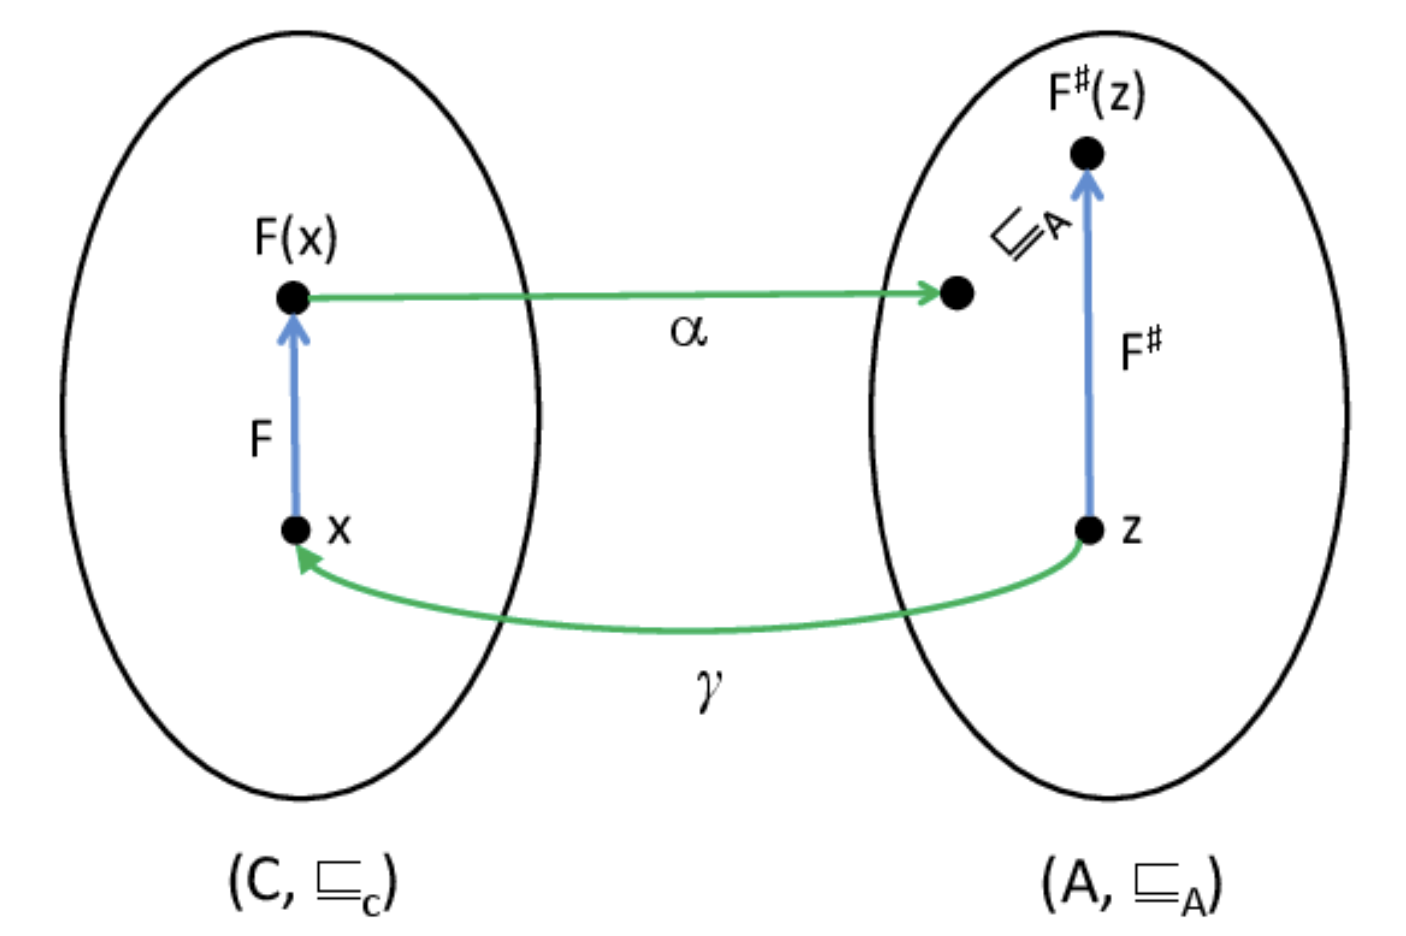
\includegraphics[width=0.7\columnwidth]{assets/approximation}
\end{center}

To approximate $F$, we can always define $F^\#(z) = \top$. This solution is always sound, however it is too imprecise. \\

The most precise approximation is given by $F^\#(z) = \alpha(F(\gamma(z)))$. The problem is that we often cannot implement such a $F^\#(z)$. However, we can come up with a $F^\#(z)$ that has the same behavior but a different implementation. Any such $F^\#(z)$ is referred to as the best transformer. \\

\textbf{Least Fixed Point Approximation} - If we have the following properties:
\begin{enumerate}
	\item monotone functions $F: C \to C$ and $F^\#: A \to A$
	\item $\alpha: C \to A$ and $\gamma: A \to A$ form a Galois Connection
	\item $\forall z \in A: \alpha(F(\gamma(z))) \sqsubseteq_A F^\#(z)$ (that is, $F^\#$ approximates $F$)
\end{enumerate}

Then $\alpha(\text{lfp}(F)) \sqsubseteq_A \text{lfp} (F^\#)$. This is important as it goes from local function approximation to global approximation. \\

If $\alpha$ and $\gamma$ do not form a Galois connection, then we can use the following definition of approximation: 
$$\forall z \in A : F(\gamma(z)) \sqsubseteq_C \gamma(F^\#(z))$$
\begin{center}
	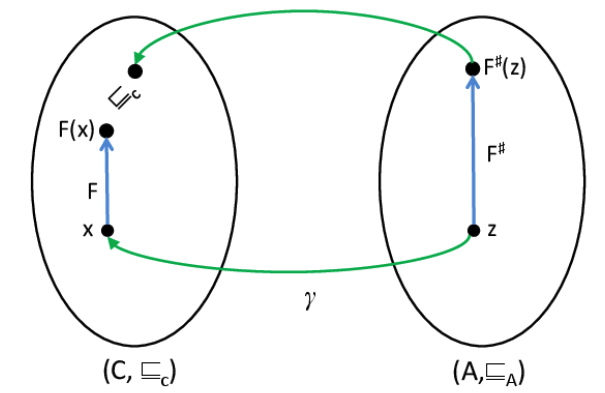
\includegraphics[width=0.7\columnwidth]{assets/approximation2}
\end{center}

If we have the following properties:
\begin{enumerate}
	\item monotone functions $F: C \to C$ and $F^\#: A \to A$
	\item $\gamma: A \to A$ is monotone
	\item $\forall z \in A : F(\gamma(z)) \sqsubseteq_C \gamma(F^\#(z))$ (that is, $F^\#$ approximates $F$)
\end{enumerate}

Then $\text{lfp}(F) \sqsubseteq_C \gamma(\text{lfp}(F^\#))$ \\

So what is $F^\#$ then? $F^\#$ is to be defined for the particular abstract domain $A$. The domain $A$ can be Sign, Parity, Interval, Polyhedra, and so on. In our setting, we simply keep a map from every label in the program to an abstract element in $A$. Then $F^\#$ simply updates the mapping from labels to abstract elements.
$$F^\#: (\text{Lab} \to A) \to (\text{Lab} \to A)$$


\subsection{Applications of Analysis: Intervals}

In this part, we will put these things together to build static analyzers. For this we first select a abstract domain, define the abstract semantics and then iterate the abstract transformer over a program until a fixed point is reached. \\

Our starting point is a domain where each element of the domain is a set of states. The domain of states is a complete lattice:
$$(\mathcal{P}(\Sigma), \subseteq, \cup, \cap, \emptyset, \Sigma) \qquad \Sigma = \text{Lab} \times \text{Store}$$

\subsubsection{Select Abstract Domain}

If we are interested in properties that involve the range of values that a variable can take, we can abstract the set of states into a map that captures the range of values each variable can take. \\

Let the interval domain be:
$$(L^i, \sqsubseteq_i, \sqcup_i, \sqcap_i, \bot_i, [-\infty, \infty])$$

We denote $\mathbb Z^\infty = \mathbb Z \cup \{-\infty, \infty\}$ and $L^i = \{ [x, y] \, | \, x, y \in \mathbb Z^\infty, x \leq y \} \cup \{ \bot_i \}$. Further we define a max and min function. Lastly, we can define the operations:
\begin{itemize}
	\item $[a, b] \sqsubseteq_i [c, d]$ if $c \leq a$ and $b \leq d$
	\item $[a, b] \sqcup_i [c, d] = [\text{min}(a, c), \text{max}(c, d)]$
	\item $[a, b] \sqcap_i [c, d] = \text{wdi}[\text{min}(a, c), \text{max}(c, d)]$ where wdi (well-defined interval) returns $[a, b]$ if $a \leq b$
\end{itemize}

The $L^i$ domain defines intervals, but to apply it we need to take program labels and program variables into account. Therefore, for programs, we use the domain: Lab $\to$ (Var $\to$ $L^i$). This domain is also a complete lattice. The operators are lifted directly to both domains.
$$\alpha_i: \mathcal P (\Sigma) \to (\text{Lab} \to (\text{Var} \to L^i))$$
$$\gamma_i: (\text{Lab} \to (\text{Var} \to L^i)) \to \mathcal P (\Sigma)$$

Using $\alpha_i$, we abstract a set of states into a map from program labels to interval ranges for each variable. Using $\gamma_i$, we concretize the intervals maps to a set of states.

\subsubsection{Define Abstract Semantics}

We still need to compute $\alpha_i [[P]]$ or an over approximation of it. We want a function: 
$$F^i: (\text{Lab} \to (\text{Var} \to L^i)) \to (\text{Lab} \to (\text{Var} \to L^i))$$

With the property $\alpha_i (\text{lfp F}) \sqsubseteq \text{lfp} F^i$. \\

\textbf{Generic Template for $F^\#$}:
$$F^\# (m) l = \begin{cases}
	\top & \text{if } l \text{ is initial label} \\
	\bigsqcup_{(l', \text{action}, l)} [[\text{action}]](m(l')) & \text{otherwise}
\end{cases}$$

This results in the following $F^i$ which approximates the best transformer but only works on the abstract domain.
$$F^i (m) l = \begin{cases}
	\lambda v. [-\infty, \infty] & \text{if } l \text{ is initial label} \\
	\bigsqcup_{(l', \text{action}, l)} [[\text{action}]]_i (m(l')) & \text{otherwise}
\end{cases}$$

$(l', \text{action}, l)$ are the edges in the CFG, an example could be $(1, \text{ x := 5}, \, 2)$. Next we would need to define all the effects for these. 
\begin{center}
	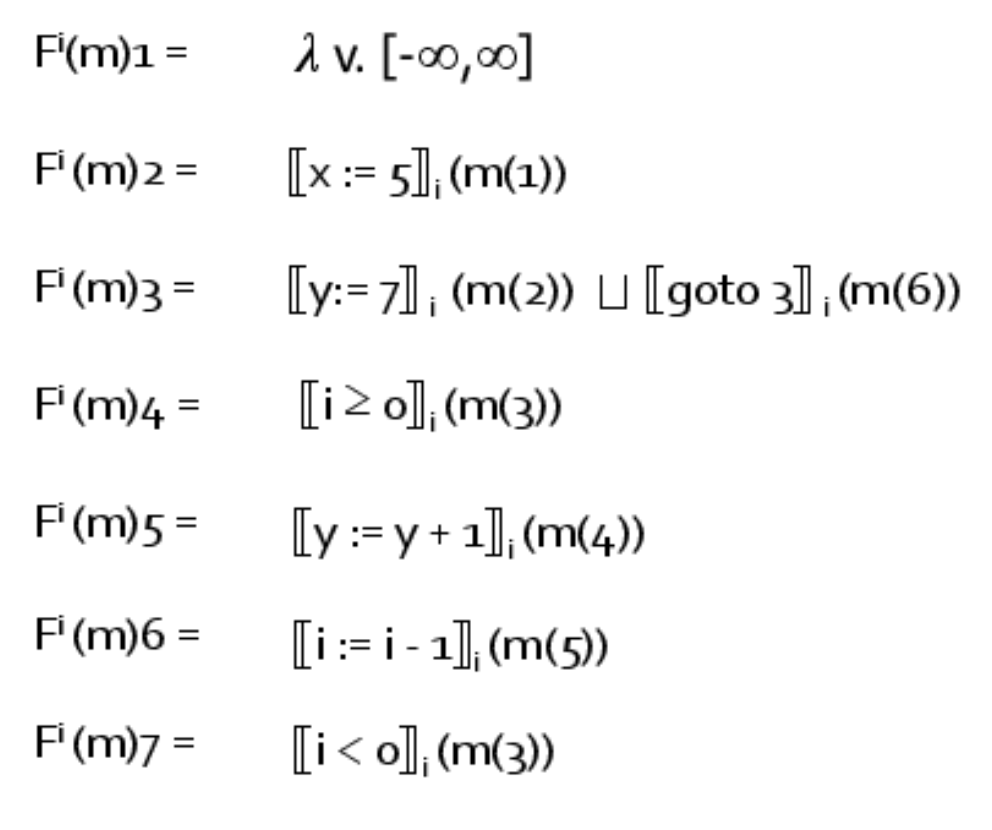
\includegraphics[width=0.6\columnwidth]{assets/effects}
\end{center}

\subsubsection{Iterate the Transformer}

In the final step, we know compute the least fixed point for a given program. However, especially with loops we can encounter the problem where a variable indefinitely changes (counts up or down). To avoid this we have to use widening. The widening operator $\nabla: L \times L \to L$ is defined as:
\begin{itemize}
	\item $\forall a,b \in L: a \sqcup b \sqsubseteq a \nabla b$
	\item if $x^0 \sqsubseteq x^1 \sqsubseteq ... \sqsubseteq x^n \sqsubseteq ...$ is an increasing sequence then $y^0 \sqsubseteq y^1 \sqsubseteq ... \sqsubseteq y^n$ stabilizes after a finite number of steps
\end{itemize}

Note that widening is completely independent of $F^i$, similar to join it is defined for a specific domain. If $\nabla, F$ are monotone then the sequence $y^0 = \bot, y^1 = y^0 \nabla F(y^0), ...$ will stabilize after a finite number of steps $n$ with $y^n$ being a post-fixed point of $F$. \\

For the interval domain, we define the widening operator $\nabla_i$ as $[a, b] \nabla_i [c, d] = [e, f]$ where $e = -\infty$ if $c < a$ and $f = \infty$ if $b < d$. \\

Iteration does not have to be in-order, there is also chaotic (asynchronous) iteration.


\subsection{Applications of Analysis: Pointers}

Pointer and Alias Analysis is fundamental to reasoning about heap manipulation programs. First we define the concrete store:
\begin{itemize}
	\item Objs is the set of all possible objects
	\item PtrVal = Objs $\cup \, \{$null$\}$
	\item $p \in \text{PrimEnv} : \text{Var} \to Z$
	\item $r \in \text{PtrEnv} : \text{PtrVar} \to \text{PtrVal}$
	\item $h \in \text{Heap} : \text{Objs} \to (\text{Field} \to \{ \text{PtrVal} \cup Z \})$
\end{itemize}

A store is now: 
$$\sigma = <p, r, h> \in \text{Store} = \text{PrimEnv} \times \text{PtrEnv} \times \text{Heap}$$

Before the store was only $p$. As before we have: 
$$\Sigma = \text{Lab} \times \text{Store}$$

Aliases are two pointers p and q that point to the same object. A points-to pair (p, A) means that p holds the address of object A. If (p, A) and (r, A) are points-to pairs, then p and r are aliases.\\

A program can create an unbounded number of objects. Therefore we need to use some abstraction when allocating a new object. That is, we need some static naming scheme for dynamically allocated objects. \\

Allocation sites divide the heap into a fixed partition based on the statement label. All objects allocated at the same program point (label) get represented by a single abstract object.
\begin{center}
	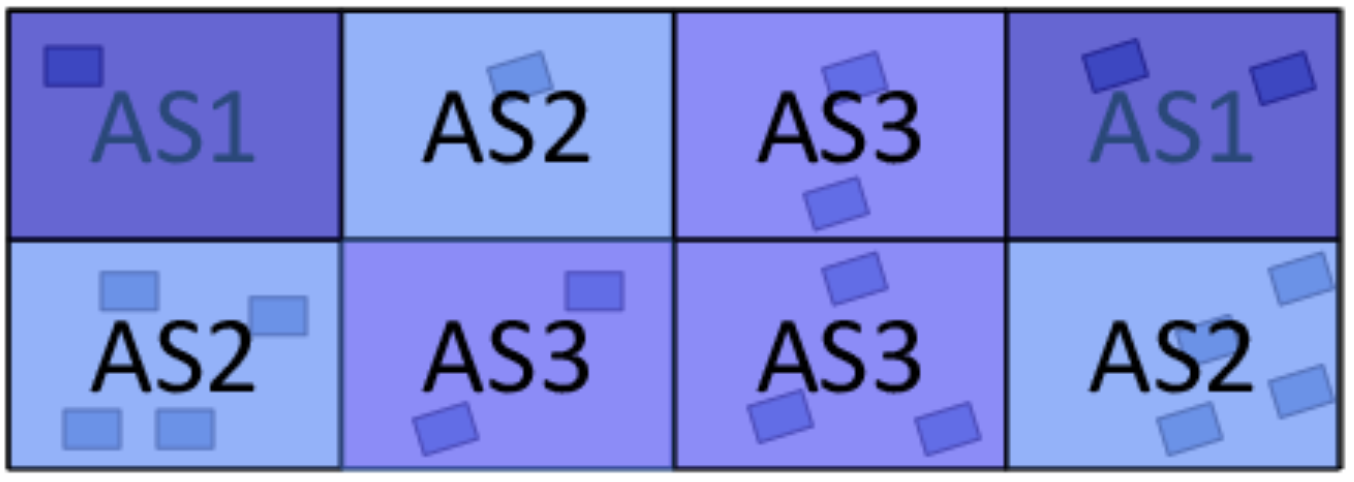
\includegraphics[width=0.8\columnwidth]{assets/allocation_sites}
\end{center}

If this is too imprecise, we can also use the calling context. If we use allocation sites (labels), we can now define the abstract objects as:
$$\text{AbsObj} = \{ l \,|\, \text{statement is p := alloc}^l \}$$

That is, this is just those labels in the program where allocation of an object occurs. Here alloc$^l$ is just the name of the allocation instruction.

\subsubsection{Flow Sensitive Pointer Analysis}

This type of analysis respects the program control flow. This leads to a separate set of points-to pairs for every program point. Further, the set at a program point represents possible maybe-aliases on some path from entry to the program point. \\

We use the same step-by-step approach as before. The abstract domain is a complete lattice:
\begin{align*}
	\text{Labs} \to ( \; &(\text{PtrVar} \to \mathcal P ( \text{AbsObj})) \; \times \\
	&( \text{AbsObj} \times \text{Field} \to \mathcal P (\text{AbsObj})) \; )
\end{align*}

The abstract domain keeps two maps at every program label. The first one contains a mapping from a pointer variable to a set of abstract objects. The second map contains a mapping from the fields of abstract objects to the set of abstract objects they point to. Since this lattice is of finite height, we will not need widening. $\sqsubseteq, \sqcup, \sqcap, \bot, \top$ are all lifted appropriately. \\

Using $\alpha$, we abstract a set of states into the two kinds of maps. Similarly, using $\gamma$, we concretize the pointer maps to a set of states. \\

We now need to define the effect of program statements manipulating pointers on the abstract domain. It can be summarized as:
\begin{center}
	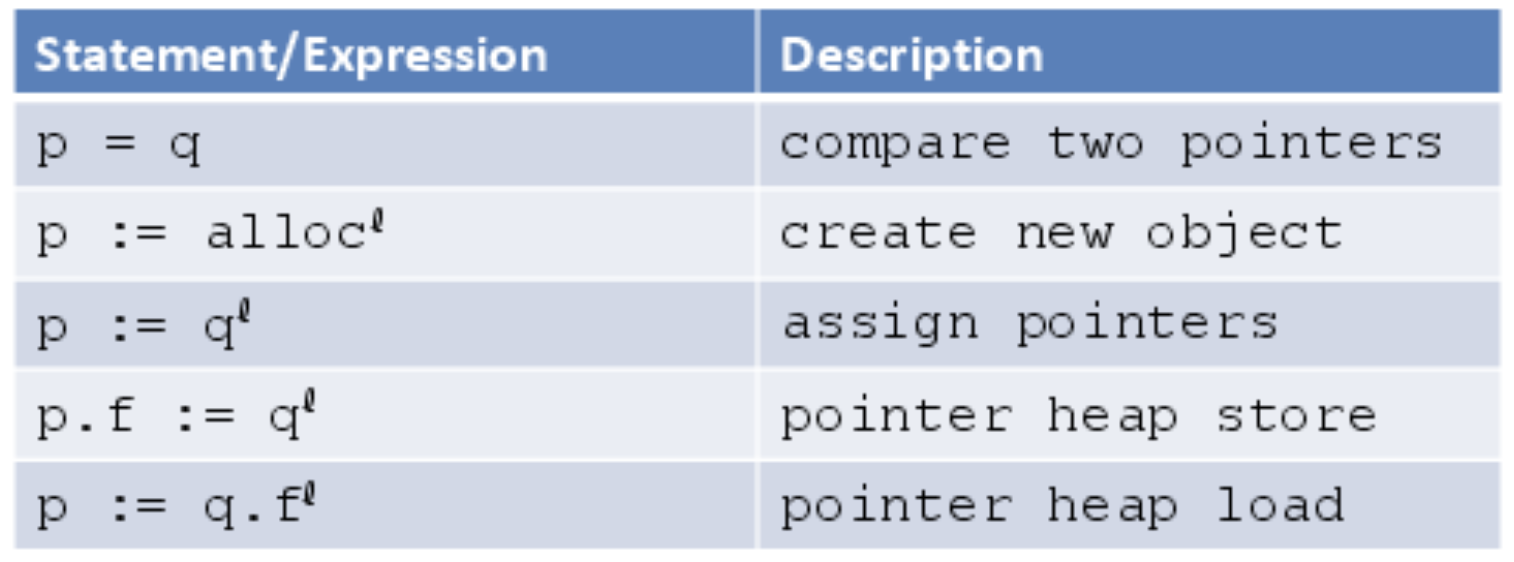
\includegraphics[width=\columnwidth]{assets/transformers}
\end{center}

Let ustake a look at the most tricky one, pointer heap store. Given \texttt{p.f := q} and \texttt{p $\to$ \{A\}}, \texttt{A.f $\to$ \{B\}}, and \texttt{q $\to$ \{C\}}. Is \texttt{A.f $\to$ \{C\}} the correct result? No, it is not. The correct solution would be \texttt{A.f $\to$ \{B, C\}}, this is called weak updates.


\subsubsection{Flow Insensitive Pointer Analysis}

This type of analysis assumes all execution orders are possible, it abstracts away order between statements. This is good for concurrency and is scalable, but it may be too imprecise. \\

The abstract domain does not keep information per label, essentially ignoring the control flow of the program.
\begin{align*}
	&(\text{PtrVar} \to \mathcal P ( \text{AbsObj})) \; \times \\
	&( \text{AbsObj} \times \text{Field} \to \mathcal P (\text{AbsObj}))
\end{align*}

To account for the loss of control-flow, all updates have to be weak. This can lead to very imprecise results. To avoid this, we can initialize local variables with \texttt{null} instead of $\top$.


\subsection{Application of Analysis: \\ Static Concurrency Checker}

Another use case is to check if parallel algorithms are deterministic. However, since proving determinism is hard, we prove a stronger property. We prove data-race freedom. \\

For static analysis there are three sources of unboundedness we have to deal with. These are the heap, the range of array indices, and the number of threads. For the heap we can use flow-insensitive points-to analysis and for the range of array indices we use numerical abstraction. \\

We first perform sequential analysis on a per thread basis. We then take the cartesian product of these states and filter out all the ones that are not possible. Leaving us with the concrete program states. \\

Now, we can check the property we are interested in proving.